\documentclass[aspectratio=169]{beamer}

% ----------------- Engine & fonts (XeLaTeX or LuaLaTeX) -----------------
\usepackage{fontspec}
\defaultfontfeatures{Ligatures=TeX}
% Formal serif text + math
\setmainfont{Libertinus Serif}
\setsansfont{Libertinus Sans}
\usepackage{mathtools}
\usepackage{bm}
\usepackage{unicode-math}
\usepackage{graphicx}
\setmathfont{Libertinus Math}
\newcommand{\Ind}[1]{\mathbb{1}\!\left[ #1 \right]}

% ----------------- Beamer look -----------------
\usetheme[progressbar=frametitle,numbering=none]{metropolis}
\setbeamertemplate{footline}[frame number]
\setbeamertemplate{navigation symbols}{}
\setbeamersize{text margin left=10mm, text margin right=10mm}
% Typographic spacing
\linespread{1.15}
\setlength{\parskip}{0.4em}
\addtolength{\abovedisplayskip}{0.3em}
\addtolength{\belowdisplayskip}{0.3em}

% ----------------- Title (EN only) -----------------
\title{Sampling Techniques in Bayesian Inference\\[0.25ex]\large Monte Carlo and Markov Chain Monte Carlo Techniques for Bayesian Inference}
\author{}
\date{}

% ----------------- Document -----------------
\graphicspath{{assets/generated/}}
\begin{document}
	
	% Title slide
	\begin{frame}
		\titlepage
	\end{frame}
	
	
	% ---------------------------------------------------------------------------
	\section{The Sampling Problem}
	\begin{frame}{The Sampling Problem}
		\textbf{Goal:} Draw samples from a target distribution $\pi(\theta)$.
		\begin{itemize}
			\item Target may be high-dimensional or multi-modal.
			\item Normalizing constant often unknown or expensive.
			\item Direct sampling rarely available.
		\end{itemize}
		\textbf{Applications:} Bayesian inference, reliability analysis, optimization.
	\end{frame}
	
	% ---------------------------------------------------------------------------
	\section{Bayesian Inference}
	\begin{frame}{Bayesian Inference}
		Given data $D$, prior $p(\theta)$ and likelihood $p(D\mid\theta)$, the posterior is
		\[
		p(\theta\mid D) = \frac{p(D\mid\theta)\,p(\theta)}{p(D)},\qquad p(D)=\int p(D\mid\theta)p(\theta)\,d\theta.
		\]
		We often evaluate the \textbf{unnormalized posterior} $\tilde p(\theta)=p(D\mid\theta)\,p(\theta)$ up to a constant and seek samples/expectations under $p(\theta\mid D)$.
	\end{frame}
	
	% Unified view: one target for all methods
	\begin{frame}{Unified View: Sampling the Posterior}
		\begin{block}{Definition}
			\textbf{Target distribution:} $p(\theta\mid D) \propto \tilde p(\theta)=p(D\mid\theta)\,p(\theta)$. We treat $\tilde p$ as an unnormalized density.
		\end{block}
		\begin{itemize}
			\item \textbf{Acceptance--Rejection:} exact independent samples if we can find $M$ and proposal $q$ s.t. $\tilde p \le M q$.
			\item \textbf{Importance Sampling:} draw $\theta_i\sim q$ and reweight by $w_i=\tilde p(\theta_i)/q(\theta_i)$ to compute posterior expectations (optionally resample for approximate draws).
			\item \textbf{MCMC:} build a Markov chain whose stationary distribution is $p(\theta\mid D)$ (acceptance ratios use $\tilde p$ so the normalizer cancels).
		\end{itemize}
	\end{frame}
	
	% ---------------------------------------------------------------------------
	\section{Acceptance--Rejection}
	\begin{frame}{Acceptance--Rejection (AR) Sampling}
		\begin{block}{Definition}
			Find $M>0$ and proposal $q(\theta)$ such that $\tilde p(\theta) \le M\,q(\theta)$ for all $\theta$.
		\end{block}
		\begin{enumerate}
			\item Draw $\theta'\sim q(\theta)$ and $u\sim \mathrm{Uniform}(0,1)$.
			\item Accept $\theta'$ if $u \le \dfrac{\tilde p(\theta')}{M\,q(\theta')}$; otherwise reject.
		\end{enumerate}
		\textbf{Notes:} Accepted $\theta'$ are independent and identically distributed from the target; efficiency improves as $Mq$ tightly envelopes $\tilde p$.
	\end{frame}
	
	\begin{frame}{AR: Efficiency Considerations}
		\begin{itemize}
			\item Expected acceptance probability equals $Z/M$.
			\item Works best in low dimension; degrades in high dimension without good envelopes.
			\item Practicalities: adaptive envelopes; log-domain evaluations to avoid underflow.
		\end{itemize}
	\end{frame}
	
	\begin{frame}{AR: Intuition}
		\begin{itemize}
			\item View $Mq(\theta)$ as an \emph{envelope} above $\tilde p(\theta) \propto p(D\mid\theta)p(\theta)$.
			\item Sample from $q$ (easy); accept with probability $\tilde p(\theta)/(M q(\theta))$.
			\item Accepted draws are exactly distributed as the target; rejections only waste computation.
		\end{itemize}
	\end{frame}
	
	\begin{frame}{Acceptance--Rejection Example: Estimating $\pi$}
		\small
		Estimate the area of the unit disk $A=\pi$.
		\begin{itemize}
			\item Target indicator: $\tilde p(x,y)=\Ind{x^2+y^2\le 1}$ on the square $[-1,1]^2$.
			\item Proposal/envelope: uniform $q(x,y)=1/4$ on $[-1,1]^2$ with $M=1$.
			\item Accept $(x,y)\sim q$ iff $x^2+y^2\le 1$. Then $\Pr(\text{accept})=A/4=\pi/4$.
			\item Estimator: $\hat\pi=4\times(\text{acceptance rate})$ (unbiased; variance decreases with $N$).
		\end{itemize}
	\end{frame}
	
	\begin{frame}
		\begin{figure}
			\centering
			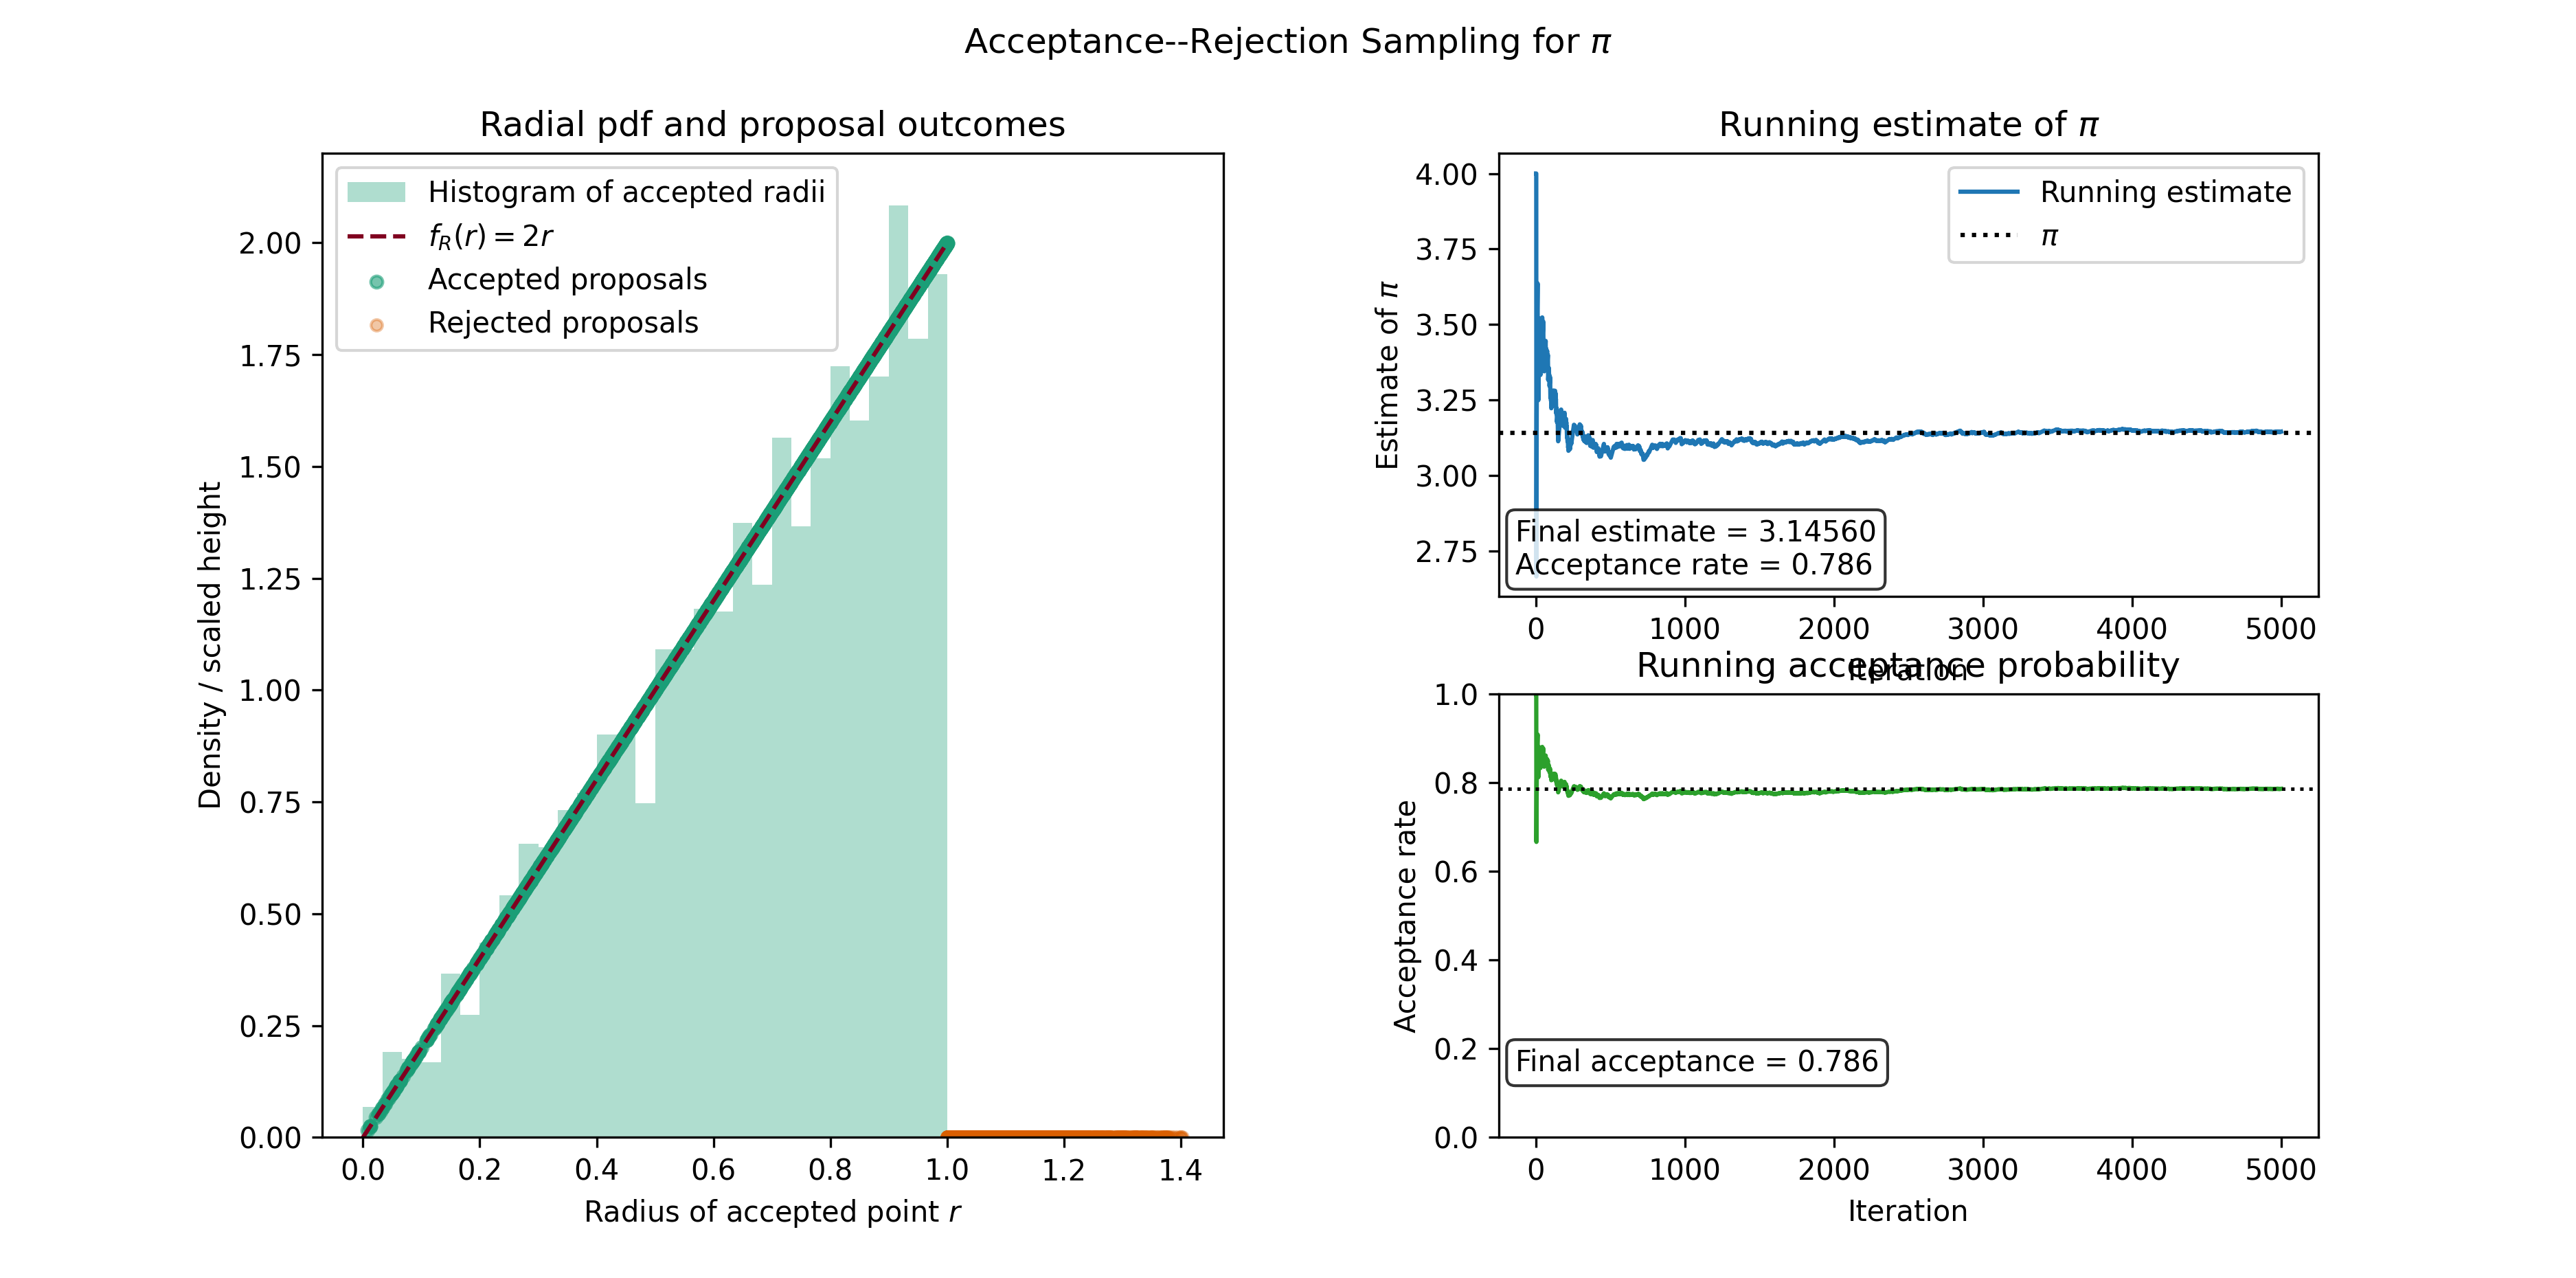
\includegraphics[width=0.9\linewidth]{ars_pi_final.png}
			\caption{Acceptance--rejection proposals and the running estimate of $\pi$.}
		\end{figure}
	\end{frame}
	
	\begin{frame}{Acceptance--Rejection Example: Beta(2,2)}
		\begin{block}{Model}
			\begin{itemize}
				\item Target $f(x)=6x(1-x)$ on $[0,1]$ (Beta$(2,2)$).
				\item Proposal $g(x)=\mathrm{Uniform}(0,1)$ with envelope constant $M=\tfrac{3}{2}$.
				\item Accept $x'$ when $u \le f(x')/(M g(x')) = 6x'(1-x')/M$.
			\end{itemize}
		\end{block}
		\begin{block}{Outcome snapshot}
			\begin{itemize}
				\item $\mathbb{P}(\text{accept}) = Z/M = 1 / (3/2) = 2/3 \approx 0.66$; simulated rate aligns with theory.
				\item $\mathbb{E}[X] = \dfrac{\alpha}{\alpha+\beta} = \tfrac{1}{2}$ and $\widehat{\mathbb{E}}[X]$ closely matches this value.
				\item $\mathbb{E}[X^2] = \dfrac{\alpha(\alpha+1)}{(\alpha+\beta)(\alpha+\beta+1)} = \tfrac{3}{10}$ and $\mathrm{Var}(X)=\dfrac{\alpha\beta}{(\alpha+\beta)^2(\alpha+\beta+1)}=\tfrac{1}{20}$, recovered by the accepted draws.
			\end{itemize}
		\end{block}
	\end{frame}
	
	\begin{frame}
		\begin{figure}
			\centering
			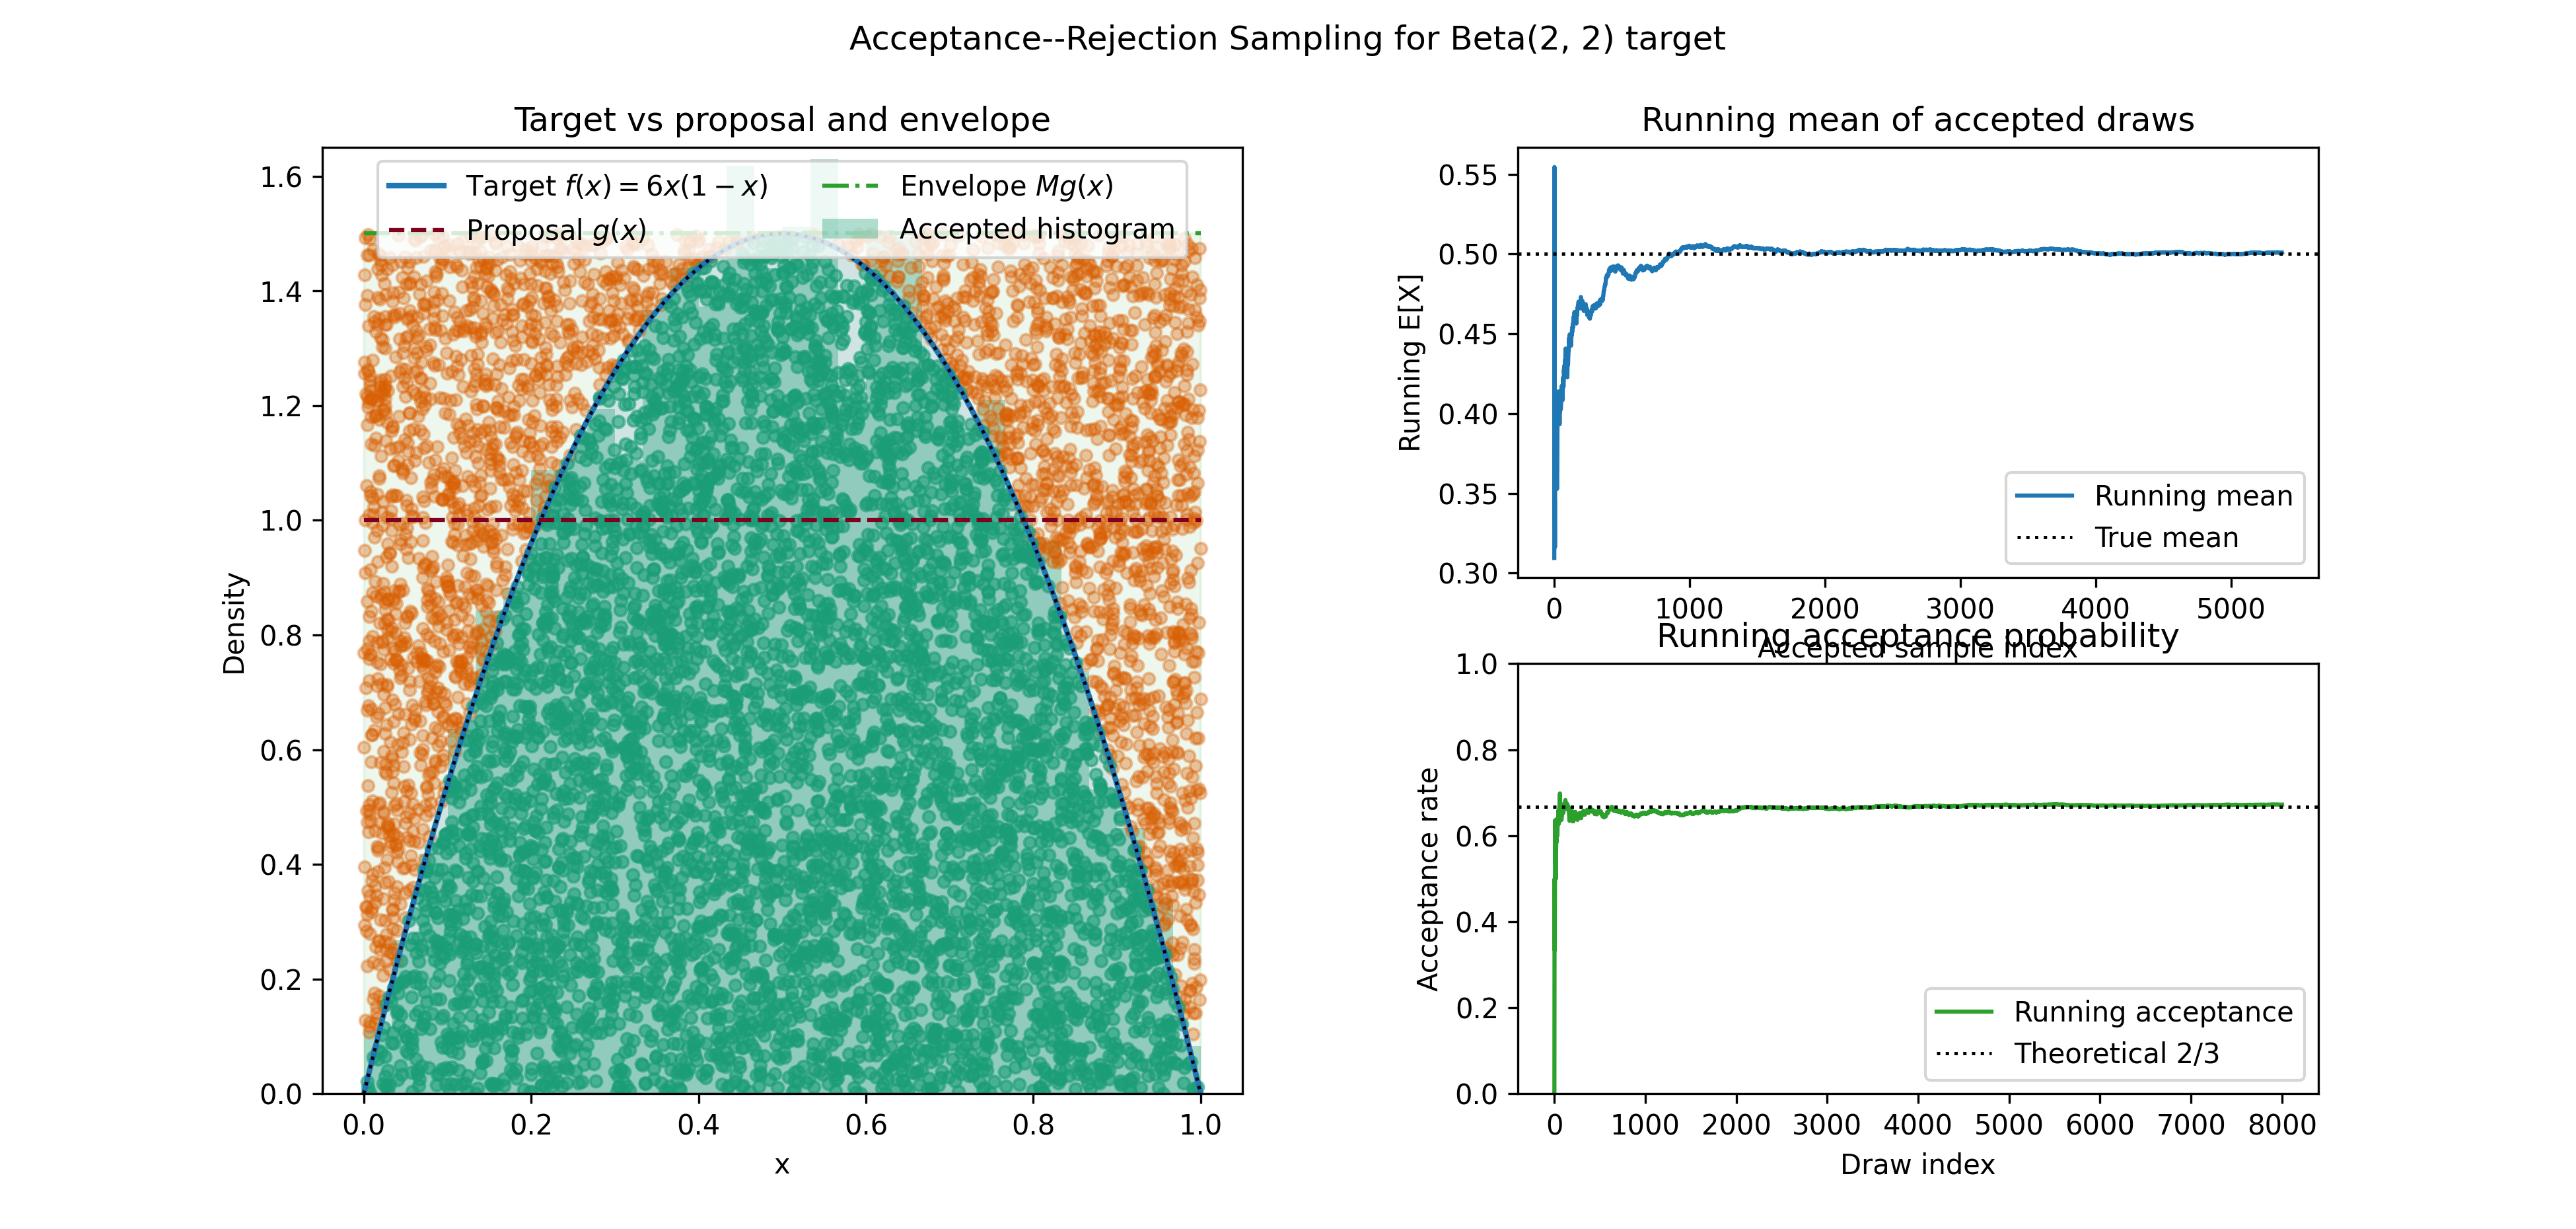
\includegraphics[width=0.9\linewidth]{ars_beta22_summary.png}
			\caption{Envelope $Mg(x)$ versus target $f(x)$ and simulated $(x,uM)$ points showing accepted (green) and rejected (orange) draws.}
		\end{figure}
	\end{frame}
	
	% ======================= Importance Sampling =======================
	\section{Importance Sampling}
	\begin{frame}{Importance Sampling: Idea}
		\begin{block}{Definition}
			For target $p(\theta\mid D) \propto \tilde p(\theta)=p(D\mid\theta)p(\theta)$ and proposal $q$, define weights $w(\theta)=\tilde p(\theta)/q(\theta)$.
		\end{block}
		We want $I=\mathbb{E}_{\pi}[f(\theta)]$ with unnormalized $\tilde p(\theta)$. Using proposal $q$:
		\[
		I=\frac{\int f(\theta)\tilde p(\theta)d\theta}{\int \tilde p(\theta)d\theta}
		=\frac{\mathbb{E}_q[f(\theta)w(\theta)]}{\mathbb{E}_q[w(\theta)]},\quad w(\theta)=\frac{\tilde p(\theta)}{q(\theta)}.
		\]
		\textbf{Support condition:} if $\tilde p(\theta)>0$ then $q(\theta)>0$.
	\end{frame}
	
	\begin{frame}{Importance Sampling: Variance, Weights, and Effective Sample Size (ESS)}
		\begin{itemize}
			\item Aim for $q$ close to $|f|\tilde p$ to reduce weight variance.
			\item \textbf{effective sample size (ESS):} $\mathrm{ESS} \approx 1/\sum_i \bar w_i^2$; report ESS/N as a diagnostic.
			\item Watch for weight degeneracy (few huge weights) $\Rightarrow$ redesign $q$.
		\end{itemize}
	\end{frame}
	
	\begin{frame}{Importance Sampling Example: Mixture Target}
		Estimate expectations under the unnormalised target $\tilde{\pi}(x) = e^{-\frac{(x-1.5)^2}{2\cdot0.6^2}} + 0.5e^{-\frac{(x+1.0)^2}{2\cdot0.9^2}}$.
		\begin{itemize}
			\item Proposal: symmetric mixture $\tilde{q}(x) = e^{-\frac{(x-1.2)^2}{2\cdot0.8^2}} + e^{-\frac{(x+1.2)^2}{2\cdot0.8^2}}$ with equal weights.
			\item Draw $x_i\sim q$ and form weights $w_i = \tilde{\pi}(x_i) / q(x_i)$ with $q$ the normalised proposal; compute $\mathbb{E}_{\pi}[f(x)] \approx \sum_i \bar w_i f(x_i)$ while monitoring ESS.
			\item Diagnostic plot: histogram shows proposal draws; scatter colour encodes normalised weights (darker points contribute more).
		\end{itemize}
	\end{frame}
	
	\begin{frame}
		\begin{figure}
			\centering
			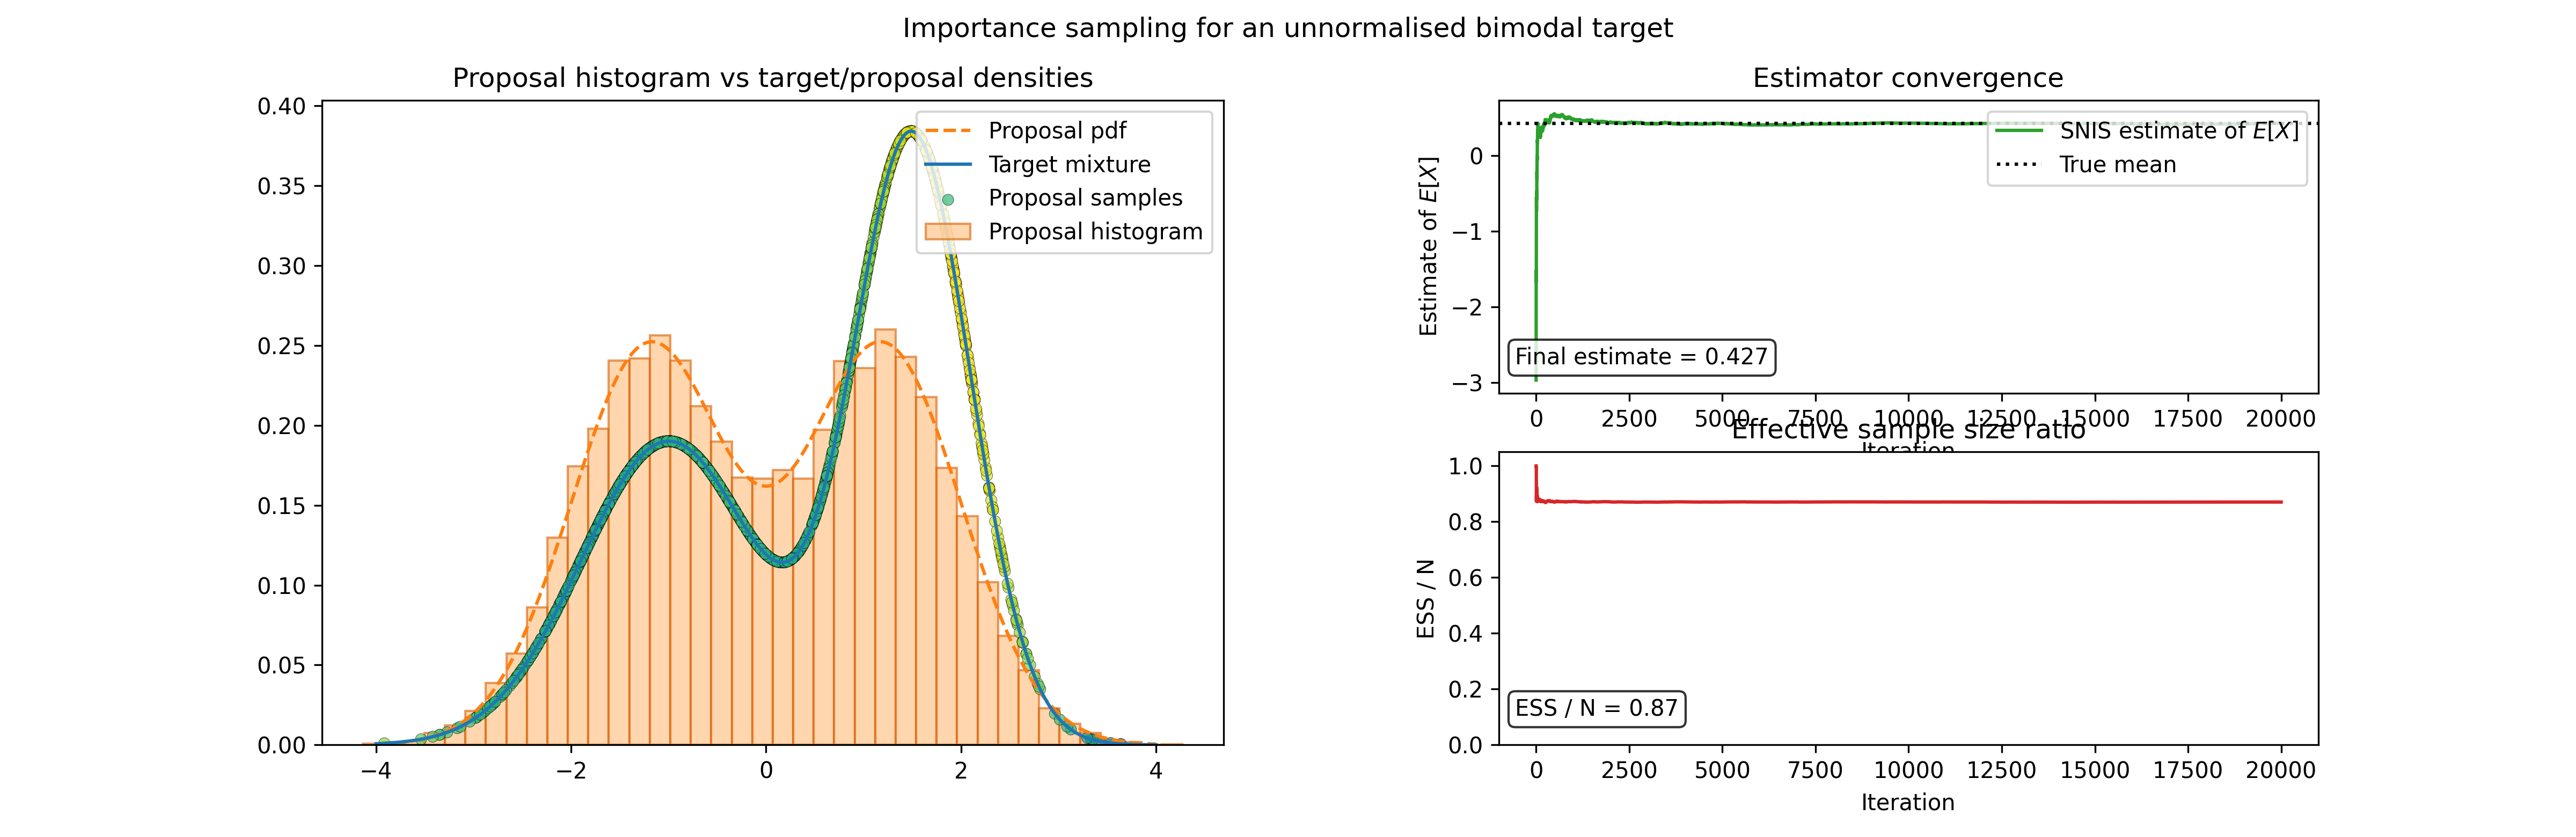
\includegraphics[width=0.9\linewidth]{is_gaussian_tail_final.png}
			\caption{Proposal histogram overlaid with target/proposal densities, weight-coloured samples, running mean, and ESS trajectory.}
		\end{figure}
	\end{frame}
	
		\begin{frame}{Importance Sampling Example: Triangular Target}
			\begin{block}{Problem setup}
				\begin{itemize}
					\item Target: triangular density on $[0,1]$ with mode $0.8$ (mean $0.6$, variance $0.0467$).
					\item Proposal: $g(x)=\mathrm{Uniform}(0,1)$ resulting in weights $w(x)=f(x)$.
					\item Quantities of interest: $\mathbb{E}[X^2]=\int_0^1 x^2 f(x)\,dx = 0.4067$ and $\Pr(X>0.9)=\int_{0.9}^1 f(x)\,dx = 0.0500$.
				\end{itemize}
			\end{block}
			\begin{block}{Outcome snapshot}
				\begin{itemize}
					\item Weighted estimates respect the integral identities above and yield ESS/N $\approx 0.75$.
					\item Unweighted uniform Monte Carlo relies on $\int_0^1 x^2 dx = \tfrac{1}{3}$ and $\int_{0.9}^1 dx = 0.1$, hence the bias relative to the target.
					\item Importance weights $w(x)=f(x)$ reweight proposals to match the desired $\mathbb{E}_f[\cdot]$ values.
				\end{itemize}
			\end{block}
		\end{frame}
	
		\begin{frame}
			\begin{figure}
				\centering
				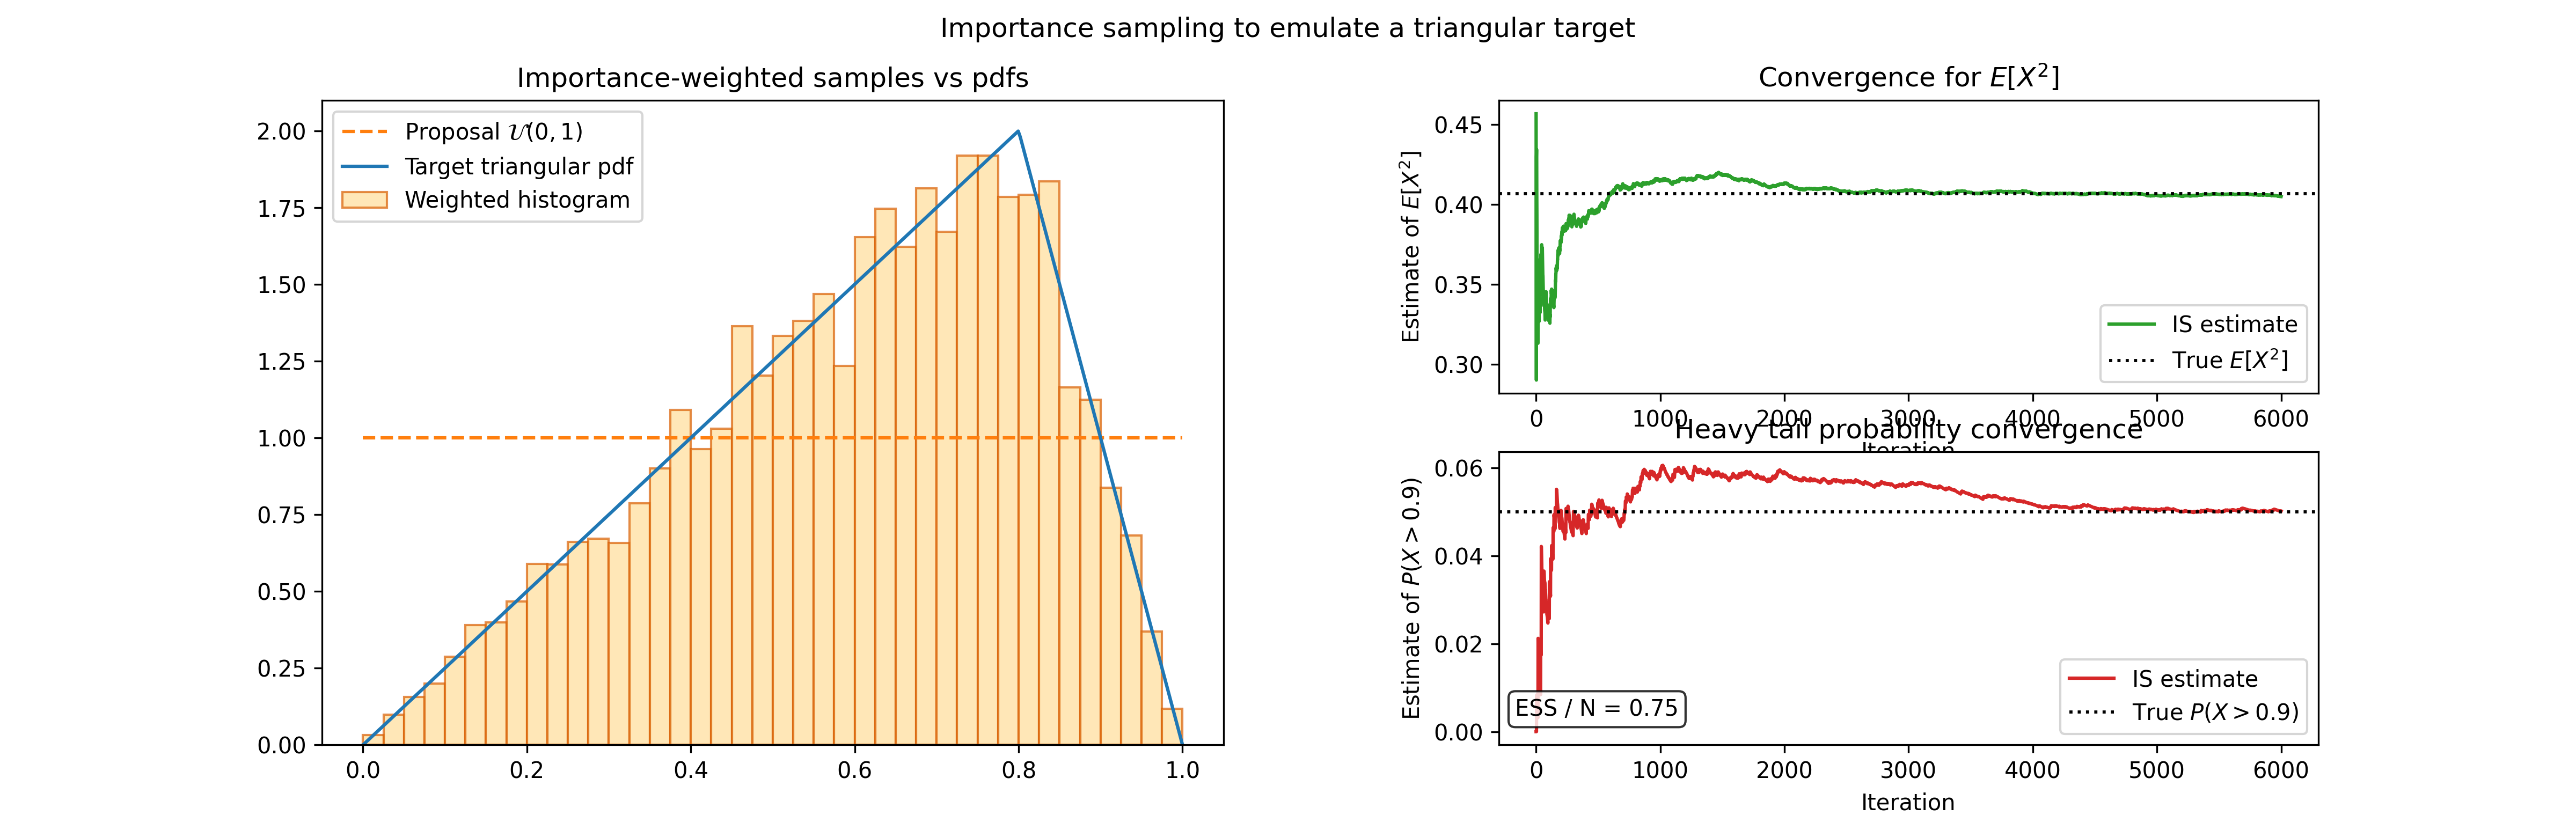
\includegraphics[width=0.9\linewidth]{is_triangular_demo.png}
				\caption{Weighted histogram, running $\mathbb{E}[X^2]$ estimate, and tail probability convergence for the triangular target.}
			\end{figure}
	\end{frame}
	
	
	% ---------------------------------------------------------------------------
	\section{MCMC Basics}
	\begin{frame}{Markov Chain Monte Carlo (MCMC)}
		\textbf{Idea:} Build a Markov chain with stationary distribution $p(\theta\mid D)$.
		\begin{itemize}
			\item Markov property: $\theta_t$ depends only on $\theta_{t-1}$.
			\item After burn-in, draws approximate posterior samples.
			\item Samples are correlated but consistent for expectations.
		\end{itemize}
	\end{frame}
	
	\begin{frame}{Key Properties}
		\begin{itemize}
			\item \textbf{Stationarity:} $\pi(\theta)$ is invariant under the transition kernel.
			\item \textbf{Ergodicity:} Time averages converge to posterior expectations.
			\item \textbf{Detailed balance} (often used): $\pi(\theta)K(\theta,\theta')=\pi(\theta')K(\theta',\theta)$.
		\end{itemize}
	\end{frame}
	
	% ---------------------------------------------------------------------------
	\section{Metropolis--Hastings}
	\begin{frame}{Metropolis--Hastings}
		\begin{block}{Definition}
			Given current $\theta$, propose a candidate $\theta'\sim q(\theta'\mid\theta)$ and accept it with probability
			\[
			\alpha(\theta,\theta') = \min\!\left(1,\; \frac{\tilde p(\theta')\,q(\theta\mid\theta')}{\tilde p(\theta)\,q(\theta'\mid\theta)}\right).
			\]
		\end{block}
		If accepted, set $\theta\leftarrow\theta'$; otherwise keep $\theta$.
	\end{frame}
	
	% Added: Metropolis--Hastings intuition, proof sketch, and figure
	\begin{frame}{Why Metropolis--Hastings Works (intuition)}
		\begin{itemize}
			\item We want a chain with stationary distribution $p(\theta\mid D)$.
			\item Propose via $q(\theta'\mid\theta)$, then \textbf{tilt} acceptance using the target density $\tilde p$.
			\item The acceptance rule balances forward and reverse moves so net probability flow cancels.
		\end{itemize}
	\end{frame}
	
	\begin{frame}{Why Metropolis--Hastings Works (sketch of proof)}
		Let $\pi(\theta)=p(\theta\mid D)$. With proposal $q$ and acceptance $\alpha$ above,
		\[
		\pi(\theta) q(\theta'\mid\theta) \alpha(\theta,\theta')
		= \min\!\Big( \pi(\theta) q(\theta'\mid\theta),\; \pi(\theta') q(\theta\mid\theta') \Big)
		= \pi(\theta') q(\theta\mid\theta') \alpha(\theta',\theta).
		\]
		Thus \textbf{detailed balance} holds and $\pi$ is stationary. Under irreducibility and aperiodicity, the chain converges to $\pi$.
	\end{frame}
	
	\begin{frame}{MCMC Example: Triangular Target}
		\begin{block}{Target density on $[0,1]$}
			\[
			f(x) = \begin{cases}
			\dfrac{2(x-0)}{(1-0)(0.8-0)}, & 0 \le x \le 0.8,\\[0.8ex]
			\dfrac{2(1-x)}{(1-0)(1-0.8)}, & 0.8 < x \le 1,\\
			0, & \text{otherwise.}
			\end{cases}
			\]
		\end{block}
		\begin{block}{Independence Metropolis--Hastings}
			\begin{itemize}
				\item Proposal $g(x)=\mathrm{Uniform}(0,1)$.
				\item Acceptance rule: $\alpha(x,x')=\min\{1, f(x')/f(x)\}$; outside $[0,1]$ proposals are rejected.
				\item Goal: approximate $\mathbb{E}_f[X]=\int_0^1 x f(x)\,dx = \frac{0+1+0.8}{3}=0.6$ and recover the target shape.
			\end{itemize}
		\end{block}
	\end{frame}
	
	\begin{frame}
		\begin{figure}
			\centering
			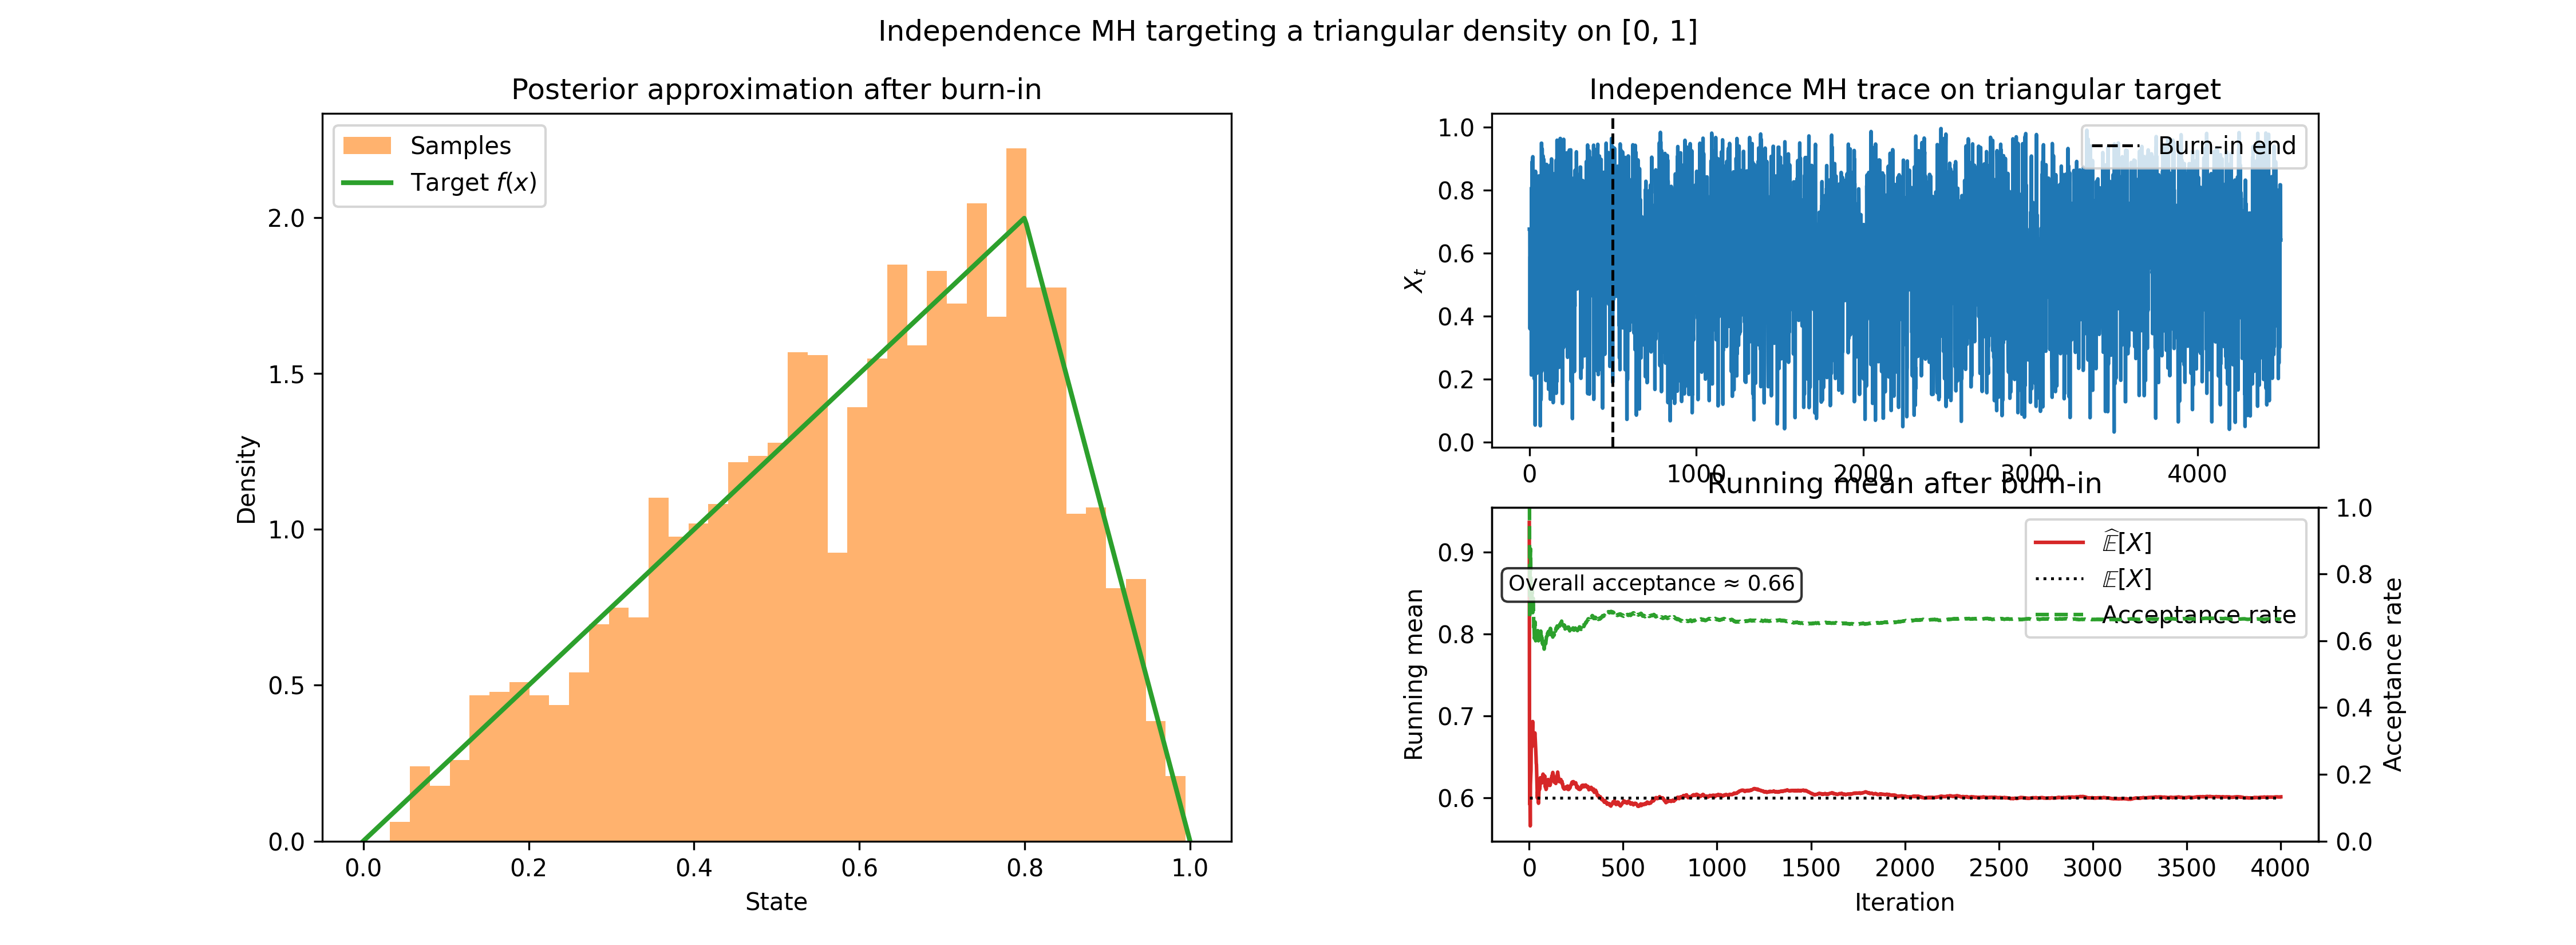
\includegraphics[width=0.9\linewidth]{mcmc_triangular_final.png}
			\caption{Trace, histogram vs.\ $f(x)$, and running mean for the independence MH sampler targeting the triangular density.}
		\end{figure}
	\end{frame}
	
	\begin{frame}{MCMC Example: Bimodal Target}
		\begin{block}{Target density}
			\[
			\pi(x)=\tfrac{1}{2}\,\mathcal{N}(x\mid -2,0.25^2) + \tfrac{1}{2}\,\mathcal{N}(x\mid 2,0.25^2).
			\]
		\end{block}
		\begin{block}{Independence MH with shared proposal}
			\begin{itemize}
				\item Proposal matches the AR envelope:
				\[
				g(x)=\tfrac{1}{2}\,\mathcal{N}(x\mid -2,1^2) + \tfrac{1}{2}\,\mathcal{N}(x\mid 2,1^2).
				\]
				\item Acceptance rule:
				\[
				\alpha(x,x')=\min\!\left\{1,\ \frac{\pi(x')/g(x')}{\pi(x)/g(x)}\right\}.
				\]
				\item Burn-in of $1{,}000$ iterations followed by $6{,}000$ retained draws; running mean quickly stabilises at $\mathbb{E}_{\pi}[X]=0$ with moderate acceptance.
			\end{itemize}
		\end{block}
	\end{frame}

	\begin{frame}
		\begin{figure}
			\centering
			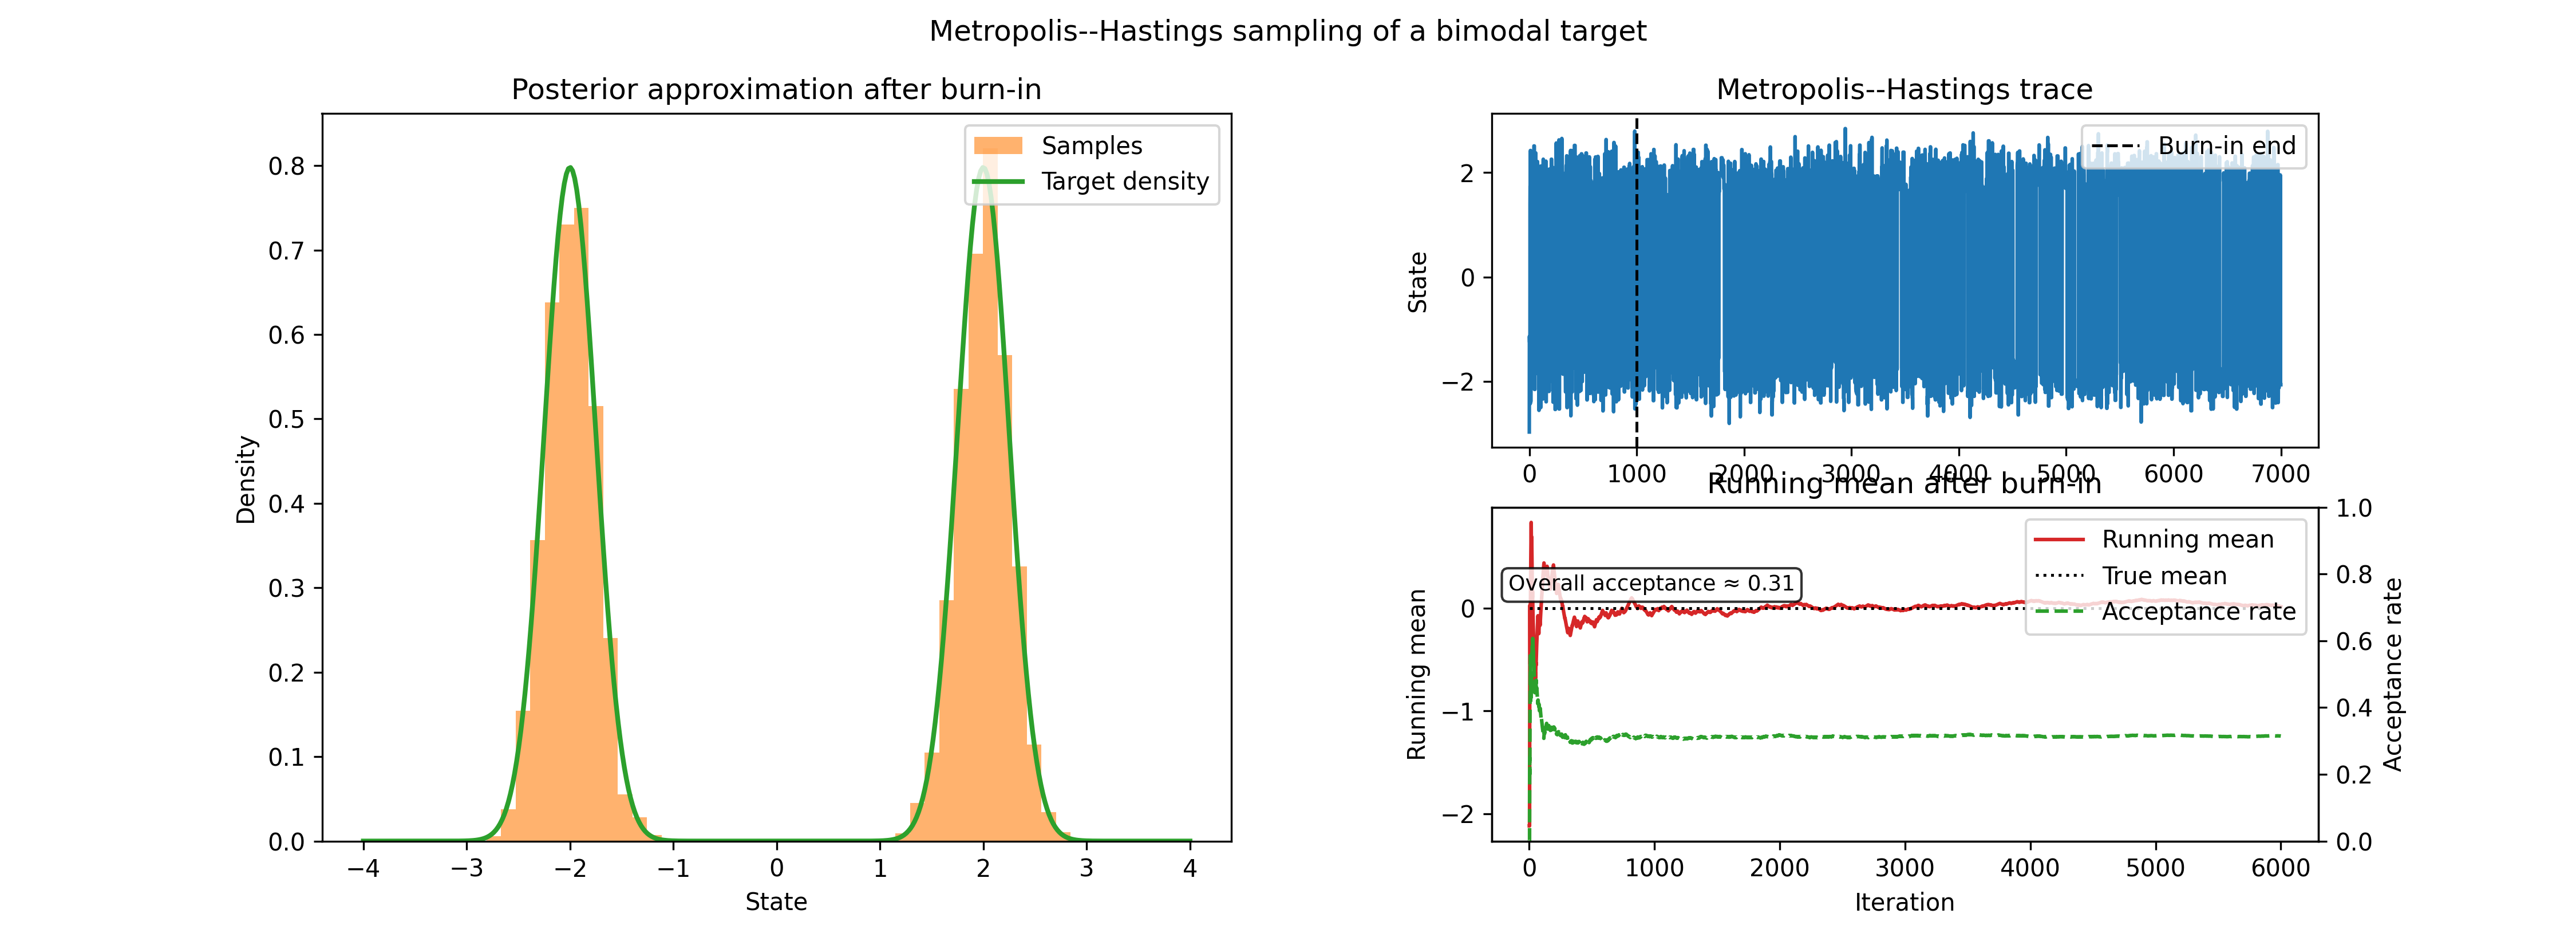
\includegraphics[width=0.9\linewidth]{mcmc_bimodal_final.png}
			\caption{Trace, histogram vs.\ $\pi(x)$, and running mean for independence MH with proposal $g(x)$ matching the AR envelope.}
		\end{figure}
	\end{frame}
	
	\begin{frame}
		\begin{figure}
			\centering
			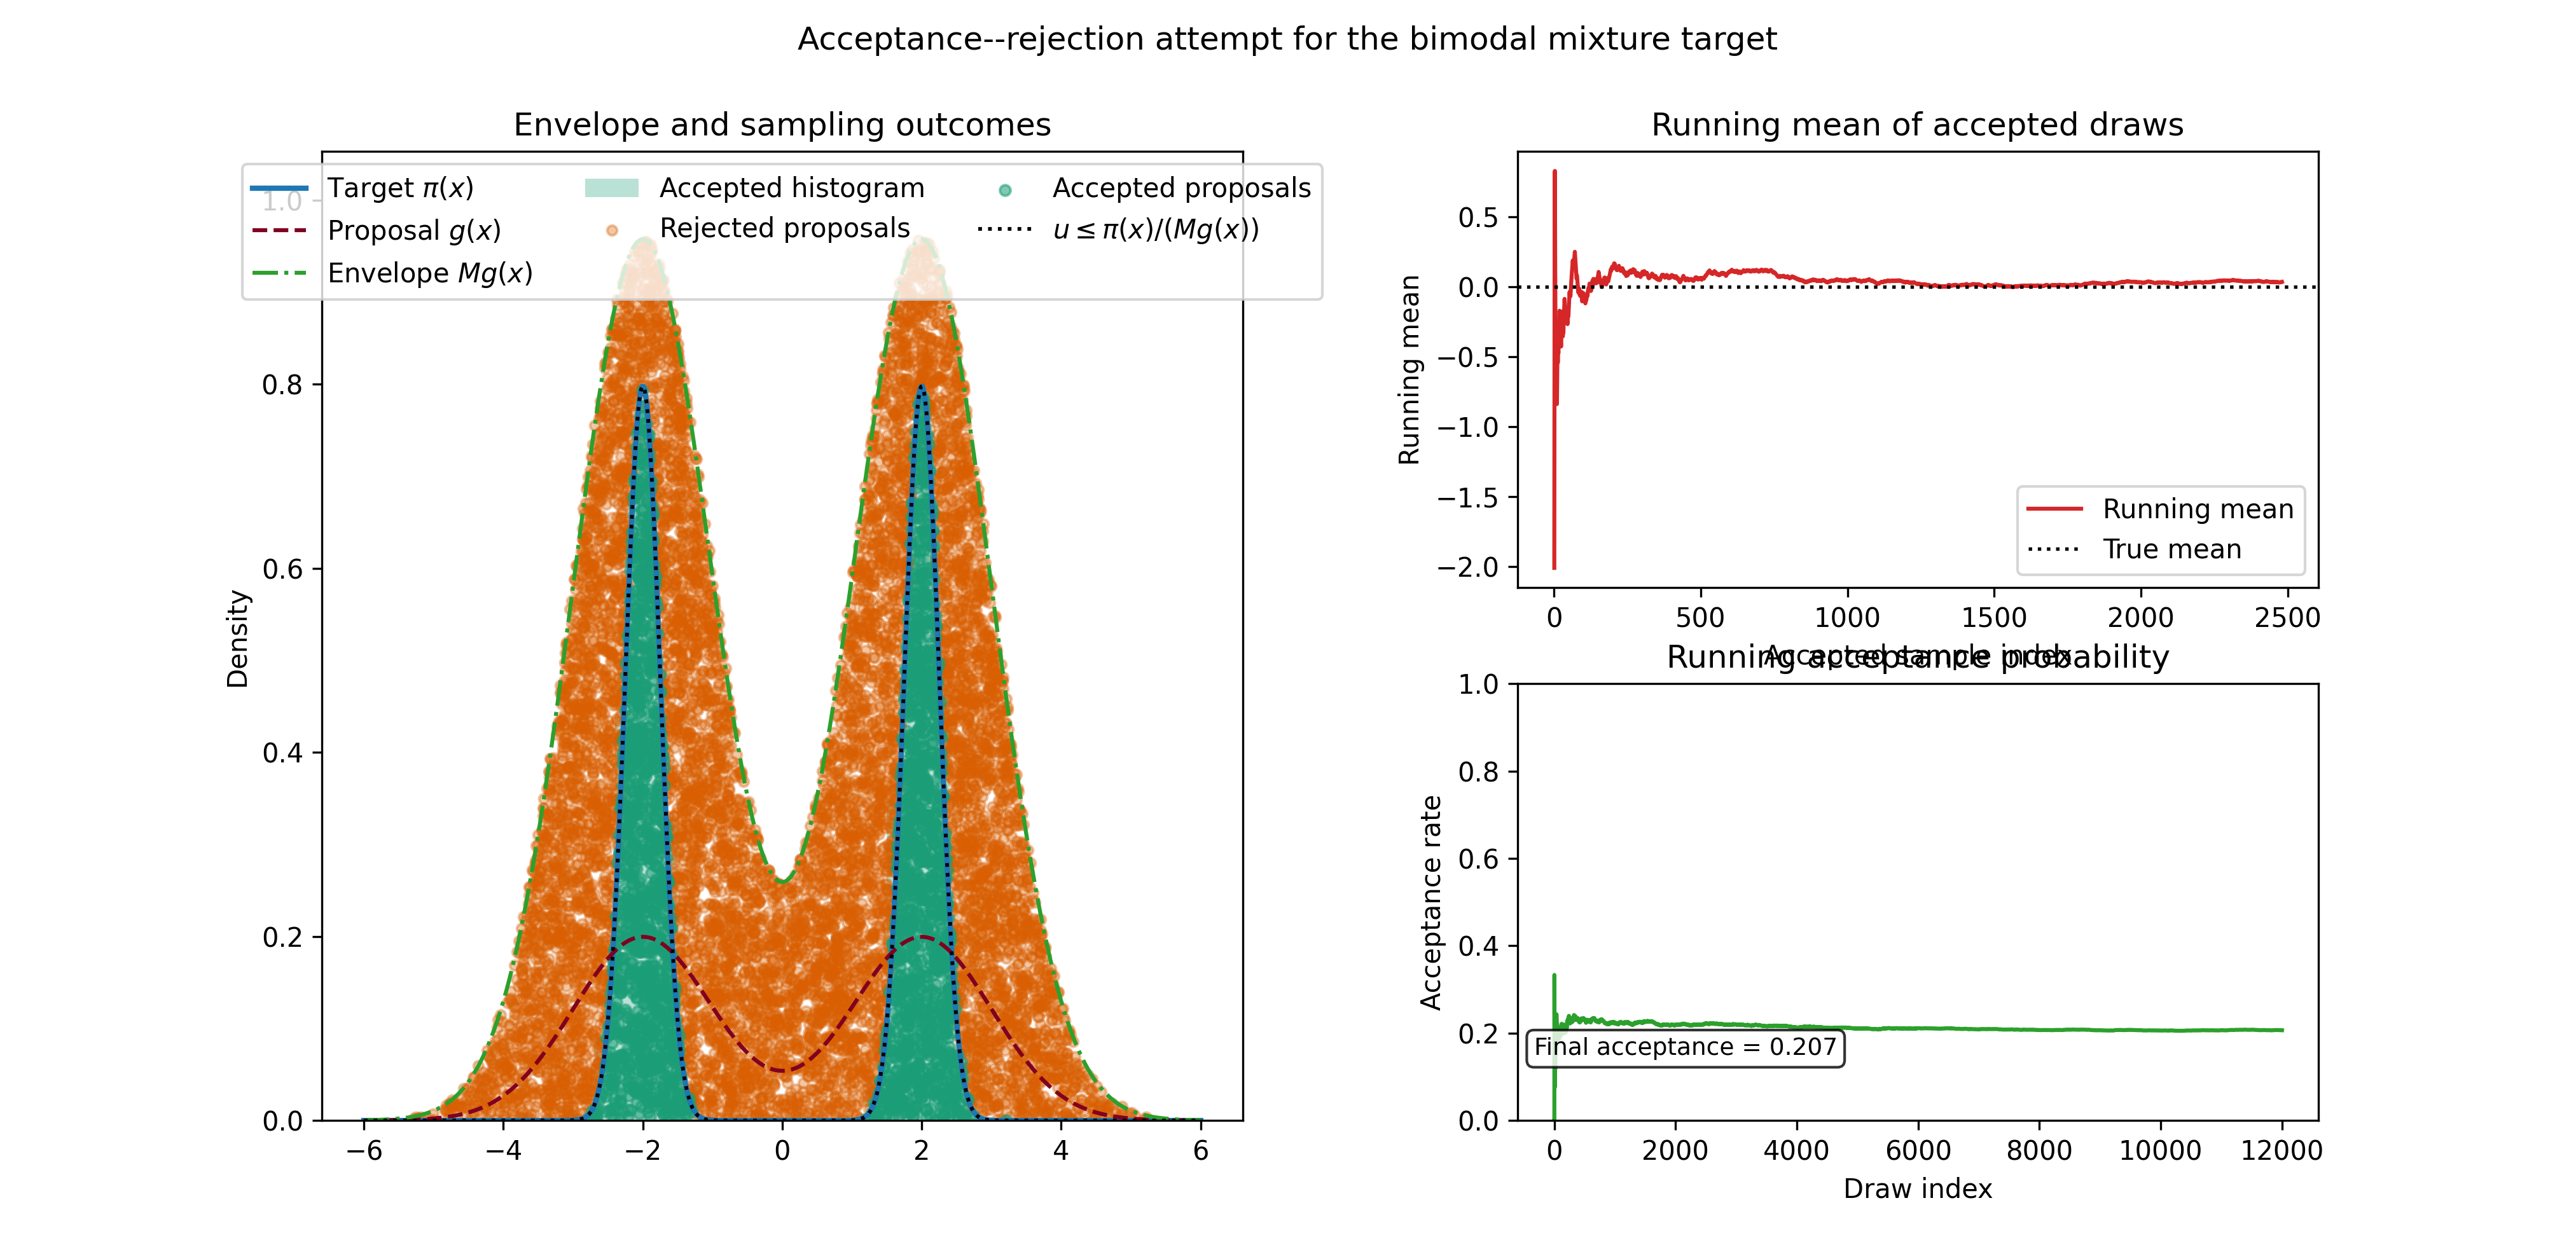
\includegraphics[width=0.9\linewidth]{ars_bimodal_comparison.png}
			\caption{Same proposal $g(x)=\tfrac{1}{2}\mathcal{N}(-2,1^2)+\tfrac{1}{2}\mathcal{N}(2,1^2)$ envelopes the sharp bimodal $\pi(x)$; low acceptance ($\approx 0.2$) slows the running mean despite i.i.d. draws.}
		\end{figure}
	\end{frame}
	
	\begin{frame}{Tuning and Diagnostics}
		\begin{itemize}
			\item Proposal scale controls acceptance rate and mixing.
			\item Monitor trace plots, autocorrelation, ESS, and $\hat R$ across chains.
			\item Burn-in to remove initialization bias; thin only if necessary for storage.
		\end{itemize}
	\end{frame}
	
	% ---------------------------------------------------------------------------
	\section{MC vs MCMC}
	\begin{frame}{Monte Carlo (MC) vs MCMC}
		\begin{itemize}
			\item \emph{MC:} Direct i.i.d. sampling when available; efficient in low dimension with tractable samplers (e.g., conjugacy, inverse-CDF).
			\item \textbf{Markov chain Monte Carlo:} Correlated chain targeting the posterior; applicable to complex or high-dimensional posteriors; requires tuning and convergence checks.
			\item MC preferred when exact/closed-form samplers exist and acceptance is high.
			\item MCMC preferred for multi-modal or high-dimensional targets when direct samplers are unavailable.
			\item Hybrids: acceptance--rejection inside Metropolis--Hastings, adaptive proposals, Hamiltonian Monte Carlo, Gibbs sampling, slice sampling.
		\end{itemize}
	\end{frame}
	
	
	% ---------------------------------------------------------------------------
	
	% ---------------------------------------------------------------------------
	
	\begin{frame}{Final Comparison: Acceptance--Rejection, Importance Sampling, Markov chain Monte Carlo}
		\begin{itemize}
			\item \textbf{Acceptance--Rejection:} independent samples; requires envelope $Mq\ge \tilde p$; strong in low dimension when $M$ is tight; acceptance $\approx 1/M$.
			\item \textbf{Importance Sampling:} estimate expectations via weighted samples; choose $q\approx |f|\tilde p$; track effective sample size and avoid weight degeneracy.
			\item \textbf{Markov chain Monte Carlo:} general-purpose for complex/high-dimensional posteriors; correlated draws; needs diagnostics ($\hat R$, effective sample size, autocorrelation).
		\end{itemize}
	\end{frame}
	
\end{document}


\begin{frame}
\frametitle{Acceptance--Rejection: Efficiency and Support}
\begin{itemize}
\item \textbf{Exact acceptance probability:} $\,\mathbb{P}(\text{accept}) = Z/M$, where $Z=\int \tilde{\pi}(\theta)\,d\theta$.
\item \textbf{Envelope condition:} Choose $M \ge \sup_{\theta} \frac{\tilde{\pi}(\theta)}{q(\theta)}$.
\item \textbf{Support condition:} Ensure $q(\theta)>0$ wherever $\tilde{\pi}(\theta)>0$.
\end{itemize}
\end{frame}

\begin{frame}
\frametitle{Importance Sampling: Essentials}
\begin{itemize}
\item \textbf{Self-normalized estimator:}
$\mathbb{E}_{\pi}[f] \approx \sum_{i=1}^N \bar w_i f(\theta_i)$,\;
$\bar w_i=\dfrac{w_i}{\sum_j w_j}$,\;
$w_i=\dfrac{\tilde{\pi}(\theta_i)}{q(\theta_i)}$.
\item \textbf{No normalizing constant needed:} Work directly with $\tilde{\pi}$; $Z$ cancels.
\item \textbf{ESS (weights):} $\mathrm{ESS} = \frac{1}{\sum_i \bar w_i^2}$.\; If $\mathrm{ESS}/N \ll 1$, redesign $q$.
\item \textbf{Tail coverage:} Choose $q$ with equal or heavier tails than $\pi$ to prevent weight explosion.
\end{itemize}
\end{frame}

\begin{frame}
\frametitle{Importance Resampling (when and how)}
\begin{itemize}
\item \textbf{When:} Trigger resampling when $\mathrm{ESS}/N$ drops below a threshold (e.g.\ 0.3--0.5).
\item \textbf{Schemes:} Multinomial, stratified, systematic; stratified/systematic reduce variance.
\item \textbf{Caveat:} Resampling yields approximately i.i.d.\ draws for simulation but can bias some estimators.
\item \textbf{Context:} This connects to Sequential Monte Carlo (SMC) when repeated over tempering/steps.
\end{itemize}
\end{frame}

\begin{frame}
\frametitle{Metropolis--Hastings: Practical Notes}
\begin{itemize}
\item \textbf{Acceptance ratio:} $\alpha(\theta,\theta')=\min\!\left(1,\,
  \frac{\tilde{\pi}(\theta')\,q(\theta\mid\theta')}{\tilde{\pi}(\theta)\,q(\theta'\mid\theta)}\right)$; the unknown $Z$ cancels.
\item \textbf{Support/irreducibility:} The proposal must eventually reach all regions with positive posterior mass.
\item \textbf{Diagnostics:} $\hat R$ for convergence across chains; time-series ESS for precision; trace/ACF plots.
\item \textbf{Thinning:} Usually unnecessary; keep all samples and rely on ESS unless storage limits require thinning.
\end{itemize}
\end{frame}

\begin{frame}
\frametitle{Reparameterizations and Jacobians}
\begin{itemize}
\item When transforming constrained parameters, include the Jacobian determinant.
\item Example (positivity): $\eta=\log\theta \Rightarrow \tilde{\pi}_\eta(\eta)=\tilde{\pi}(e^\eta)\,e^\eta$.
\item Example (simplex via softmax): $\theta_k=\frac{\exp(\eta_k)}{\sum_j \exp(\eta_j)}$; include the log-Jacobian in the target.
\end{itemize}
\end{frame}

\begin{frame}
\frametitle{Benefits of MCMC (why not plain MC)}
\begin{itemize}
\item \textbf{Flexibility:} Works with unnormalized targets $\tilde{\pi}$ where direct sampling is unavailable.
\item \textbf{Scalability:} More robust than AR/IS in moderate--high dimensions.
\item \textbf{Exploration:} Local proposals can explore complex posteriors; advanced samplers (Gibbs, HMC, slice) improve mixing.
\item \textbf{Applicability:} Handles hierarchical and constrained models via reparameterization.
\end{itemize}
\end{frame}

\begin{frame}
\frametitle{Tackling Computational Costs}
\begin{itemize}
\item \textbf{Emulators / ROMs:} Surrogates for expensive likelihoods.
\item \textbf{Parallelization:} Multiple chains, parallel proposals, tempering.
\item \textbf{Adaptive methods:} Adaptive MH, covariance adaptation; use diminishing adaptation for ergodicity.
\item \textbf{Tempering / Bridging:} AIS, SMC, parallel tempering to cross modes.
\end{itemize}
\end{frame}
